\chapter{Evaluation}
\label{ch:eval}

This chapter evaluates the two main algorithmic contributions of the pipeline: the vehicle trajectory reconstruction methods (Section~\ref{sec:eval_trace}) and the lane extraction pipeline (Section~\ref{sec:eval_lanes}).

\section{Ground Truth Collection}
\label{sec:eval_gt}

Ground truth data was manually collected for both evaluation tasks. The vehicle trajectory ground truth covers approximately $4700\,\mathrm{m}$ of the recorded highway segment. Collection was made possible by the fact that the LiDAR sensor captured a partial scan of the vehicle's trunk during every rotation. The centroids of these trunk point clusters were manually extracted and used as ground truth positions of the vehicle/sensor. Since this method need not be perfectly precise---only sufficiently accurate to serve as a reference for algorithm comparison---it provides an adequate basis for evaluation.

The lane geometry ground truth spans more than $10\,\mathrm{km}$ of annotated lane boundaries, each labeled semantically as either \emph{solid} or \emph{dashed}. The geometries were extracted based on intensity values and saved to a GeoPackage file.

%------------------------------------------------------------------
\section{Vehicle Trajectory Reconstruction Evaluation}
\label{sec:eval_trace}

\subsection{Evaluation Methodology}
\label{sec:eval_trace_method}

To quantitatively evaluate the geometric accuracy of the generated vehicle trajectories, the algorithm-produced traces were compared against the manually annotated ground-truth reference traces. The evaluation focuses on spatial similarity between the detected and reference paths and measures both average positional accuracy and worst-case deviations. The same evaluation procedure was applied to all four trajectory reconstruction methods.

\subsubsection{Spatial Alignment and Preprocessing}

Both the algorithm-generated trace and the ground-truth trace were loaded from GeoPackage files and transformed into the Hungarian projected coordinate reference system EPSG:23700. Using a projected CRS ensures that all geometric distance calculations are performed in metres.

Since the algorithms produce trajectories extending beyond the manually annotated road segment, the generated trace was spatially trimmed before comparison. The start and end points of the ground-truth trajectory were projected onto the generated polyline, and the corresponding substring was extracted. This step guarantees that both geometries represent the same road segment.

\subsubsection{Trajectory Sampling}

To enable dense geometric comparison, both polylines were sampled at regular intervals of $0.3\,\mathrm{m}$ along their lengths, producing approximately uniformly spaced points on each trajectory. Let
\begin{equation}
  G = \{g_1, g_2, \dots, g_n\}
  \label{eq:gt_samples}
\end{equation}
denote the sampled points of the ground-truth trajectory, and
\begin{equation}
  A = \{a_1, a_2, \dots, a_m\}
  \label{eq:algo_samples}
\end{equation}
the sampled points of the algorithm-generated trajectory.

\subsubsection{Bidirectional Point-to-Curve Distance Evaluation}

The evaluation computes distances in both directions:
\begin{enumerate}
  \item From every ground-truth sample point $g_i \in G$ to the generated trajectory $A$.
  \item From every generated sample point $a_j \in A$ to the ground-truth trajectory $G$.
\end{enumerate}

For a point $g_i \in G$, the distance to $A$ is defined as
\begin{equation}
  d(g_i, A) = \min_{a \in A} \|g_i - a\|,
  \label{eq:point_to_curve}
\end{equation}
and analogously for points sampled from $A$. Using bidirectional distances is important because a one-sided evaluation may fail to capture certain geometric discrepancies: a generated trajectory may fully cover the ground-truth line while also containing large overextensions elsewhere (see Figure~\ref{fig:trace_sampling}).

\begin{figure}[htbp]
  \centering
  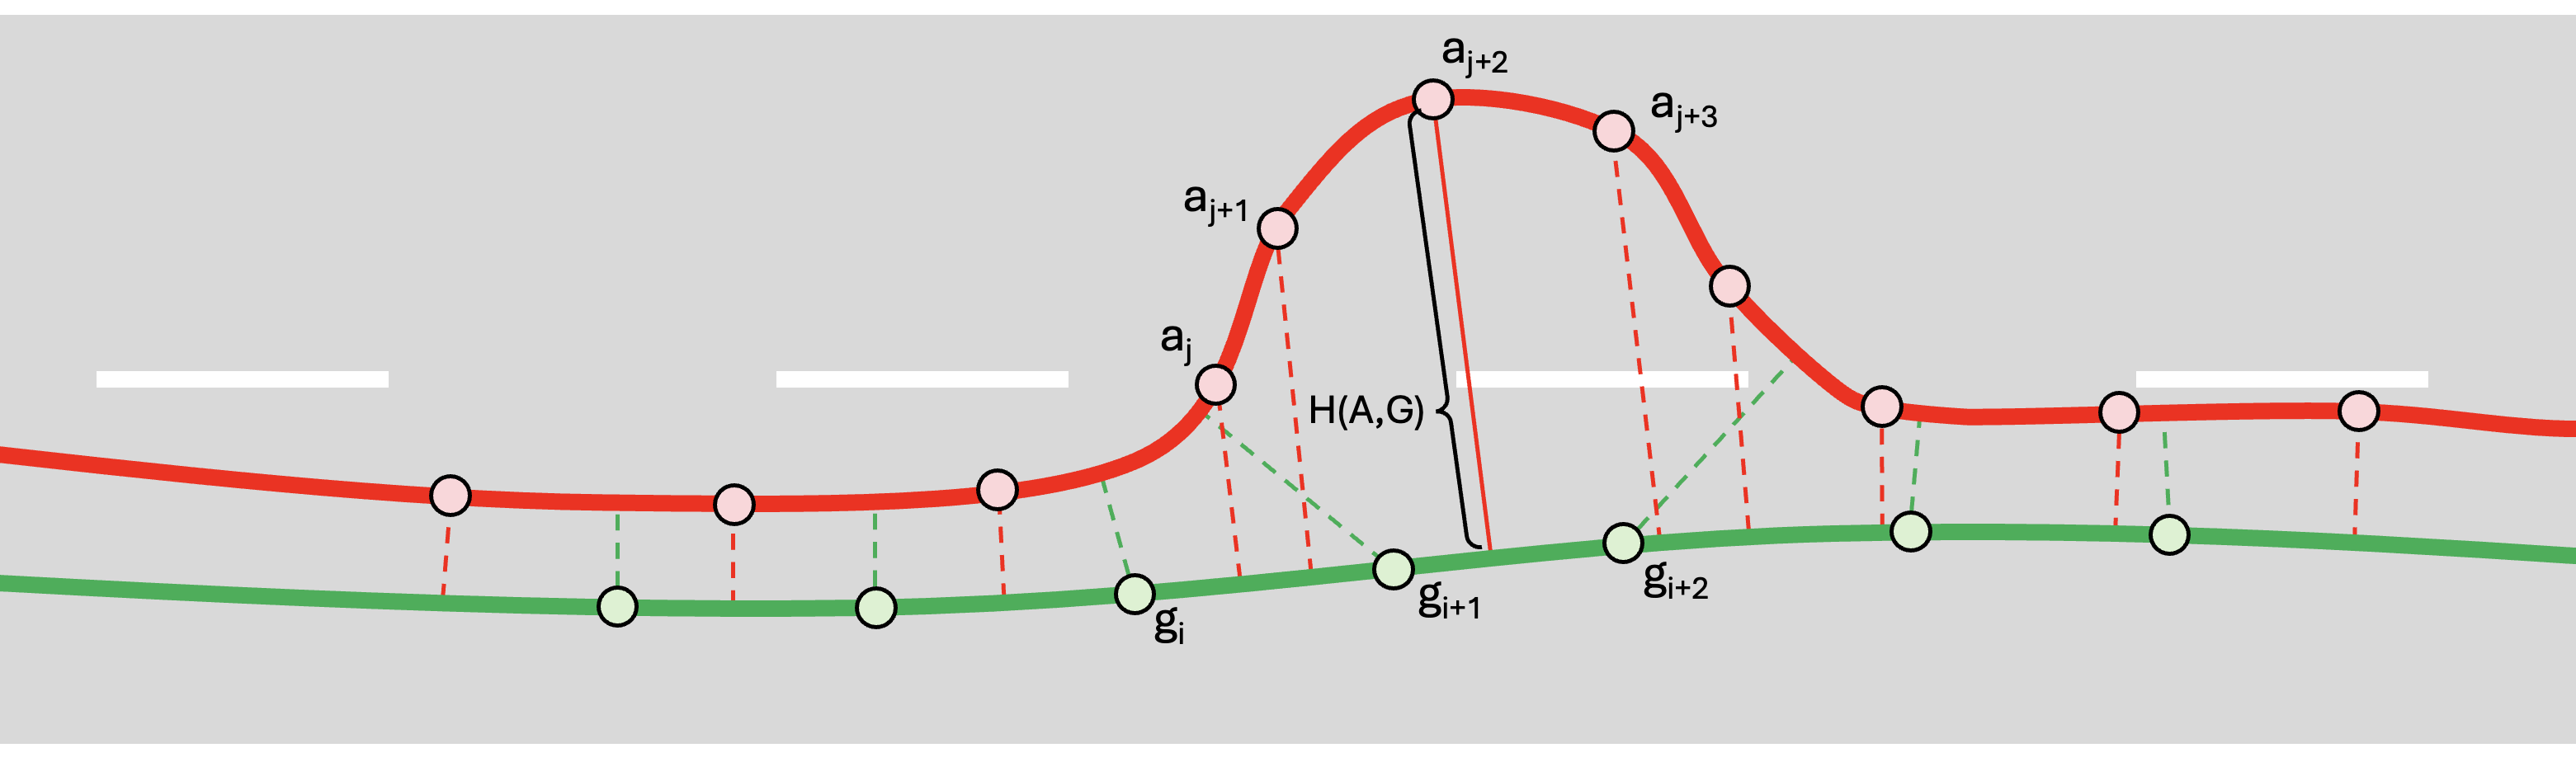
\includegraphics[width=0.8\textwidth]{images/evaluation/trace/trace_sampling}
  \caption{Illustration of the bidirectional sampling-based evaluation. Ground-truth trace (green) and algorithm trace (red) are sampled densely; shortest distances from green samples (light green) and from red samples (pink) are computed independently. The Hausdorff distance is the maximum of all shortest distances.}
  \label{fig:trace_sampling}
\end{figure}

For each direction, the following statistical measures were computed:

\begin{description}
  \item[Mean Error] Average geometric deviation between the trajectories:
    \begin{equation}
      \mu = \frac{1}{N}\sum_{i=1}^{N} d_i.
      \label{eq:mean_error}
    \end{equation}

  \item[Root Mean Square Error (RMSE)] Gives higher weight to larger local deviations:
    \begin{equation}
      \mathrm{RMSE} = \sqrt{\frac{1}{N}\sum_{i=1}^{N} d_i^2}.
      \label{eq:rmse}
    \end{equation}

  \item[95th Percentile (P95)] The distance below which $95\%$ of all sampled errors fall.

  \item[99th Percentile (P99)] Indicates the behavior of extreme outliers while remaining less sensitive than the absolute maximum.
\end{description}

\FloatBarrier
\subsection{Hausdorff Distance}
\label{sec:eval_hausdorff}

As a global similarity measure, the evaluation also computes the Hausdorff distance between the two trajectories. The directed Hausdorff distance from $A$ to $G$ is defined as
\begin{equation}
  h(A, G) = \max_{a \in A} \min_{g \in G} \|a - g\|,
  \label{eq:directed_hausdorff}
\end{equation}
and the symmetric Hausdorff distance is
\begin{equation}
  H(A, G) = \max\bigl(h(A, G),\; h(G, A)\bigr).
  \label{eq:hausdorff}
\end{equation}

Intuitively, the Hausdorff distance represents the largest local deviation between the two trajectories: it is the maximum distance that any point on one curve must travel to reach the nearest point on the other. Unlike mean-based metrics, it is highly sensitive to localized outliers and therefore provides a useful worst-case similarity measure. A small Hausdorff distance indicates that the generated trajectory remains close to the reference everywhere along its length.

\FloatBarrier
\subsection{Fréchet Distance}
\label{sec:eval_frechet}

Another commonly used curve similarity metric is the Fréchet distance, which---unlike the Hausdorff distance---takes the ordering of points along the curves into account. It is often illustrated by the analogy of a person walking a dog: both move along their respective curves without backtracking, and the Fréchet distance is the minimum leash length required. Formally, for two curves $f$ and $g$:
\begin{equation}
  F(f, g) = \inf_{\alpha,\beta}\; \max_{t \in [0,1]} \|f(\alpha(t)) - g(\beta(t))\|,
  \label{eq:frechet}
\end{equation}
where $\alpha$ and $\beta$ are continuous non-decreasing reparameterizations of the two curves.

Although the Fréchet distance is frequently used for trajectory comparison, it was not necessary in this evaluation because the trajectories contain no loops, self-intersections, or backward movements. Under such conditions, the Fréchet and Hausdorff distances tend to be very similar in practice, since both trajectories follow nearly monotonic paths with consistent ordering. In general,
\begin{equation}
  F(A, G) \geq H(A, G),
  \label{eq:frechet_hausdorff}
\end{equation}
with equality only in special cases. The Fréchet distance would therefore provide little additional information beyond the Hausdorff distance for these trajectories.

\FloatBarrier
\subsection{Evaluation Results}
\label{sec:eval_trace_results}

Tables~\ref{tab:trace_wm1}--\ref{tab:trace_cp} report the evaluation metrics for each trajectory reconstruction method. Figure~\ref{fig:trace_histograms} shows the corresponding distance distributions.

\begin{table}[htbp]
  \centering
  \caption{Window Median (Baseline) --- trajectory evaluation results.}
  \label{tab:trace_wm1}
  \small
  \begin{tabular}{@{}lrrrr@{}}
    \hline
    Direction   & Mean Error & RMSE    & P95     & P99     \\
    \hline
    GT $\to$ Algo & $0.653\,\mathrm{m}$ & $0.748\,\mathrm{m}$ & $1.252\,\mathrm{m}$ & $1.769\,\mathrm{m}$ \\
    Algo $\to$ GT & $0.653\,\mathrm{m}$ & $0.747\,\mathrm{m}$ & $1.250\,\mathrm{m}$ & $1.768\,\mathrm{m}$ \\
    \hline
    \multicolumn{2}{@{}l}{Hausdorff distance} & \multicolumn{3}{r@{}}{$1.960\,\mathrm{m}$} \\
    \hline
  \end{tabular}
\end{table}

\begin{table}[htbp]
  \centering
  \caption{Window Median with Ground Filtering (V2) --- trajectory evaluation results.}
  \label{tab:trace_wm2}
  \small
  \begin{tabular}{@{}lrrrr@{}}
    \hline
    Direction   & Mean Error & RMSE    & P95     & P99     \\
    \hline
    GT $\to$ Algo & $0.177\,\mathrm{m}$ & $0.305\,\mathrm{m}$ & $0.508\,\mathrm{m}$ & $1.527\,\mathrm{m}$ \\
    Algo $\to$ GT & $0.176\,\mathrm{m}$ & $0.303\,\mathrm{m}$ & $0.506\,\mathrm{m}$ & $1.522\,\mathrm{m}$ \\
    \hline
    \multicolumn{2}{@{}l}{Hausdorff distance} & \multicolumn{3}{r@{}}{$1.782\,\mathrm{m}$} \\
    \hline
  \end{tabular}
\end{table}

\begin{table}[htbp]
  \centering
  \caption{Pulse Line Intersection --- trajectory evaluation results.}
  \label{tab:trace_pl}
  \small
  \begin{tabular}{@{}lrrrr@{}}
    \hline
    Direction   & Mean Error & RMSE    & P95     & P99     \\
    \hline
    GT $\to$ Algo & $0.147\,\mathrm{m}$ & $0.182\,\mathrm{m}$ & $0.348\,\mathrm{m}$ & $0.439\,\mathrm{m}$ \\
    Algo $\to$ GT & $0.147\,\mathrm{m}$ & $0.183\,\mathrm{m}$ & $0.349\,\mathrm{m}$ & $0.439\,\mathrm{m}$ \\
    \hline
    \multicolumn{2}{@{}l}{Hausdorff distance} & \multicolumn{3}{r@{}}{$0.725\,\mathrm{m}$} \\
    \hline
  \end{tabular}
\end{table}

\begin{table}[htbp]
  \centering
  \caption{Closest Point Convergence (after smoothing) --- trajectory evaluation results.}
  \label{tab:trace_cp}
  \small
  \begin{tabular}{@{}lrrrr@{}}
    \hline
    Direction   & Mean Error & RMSE    & P95     & P99     \\
    \hline
    GT $\to$ Algo & $0.653\,\mathrm{m}$ & $0.748\,\mathrm{m}$ & $1.252\,\mathrm{m}$ & $1.769\,\mathrm{m}$ \\
    Algo $\to$ GT & $0.653\,\mathrm{m}$ & $0.747\,\mathrm{m}$ & $1.250\,\mathrm{m}$ & $1.768\,\mathrm{m}$ \\
    \hline
    \multicolumn{2}{@{}l}{Hausdorff distance} & \multicolumn{3}{r@{}}{$1.960\,\mathrm{m}$} \\
    \hline
  \end{tabular}
\end{table}

\begin{figure}[htbp]
  \centering
  \begin{subfigure}[b]{0.8\textwidth}
    \centering
    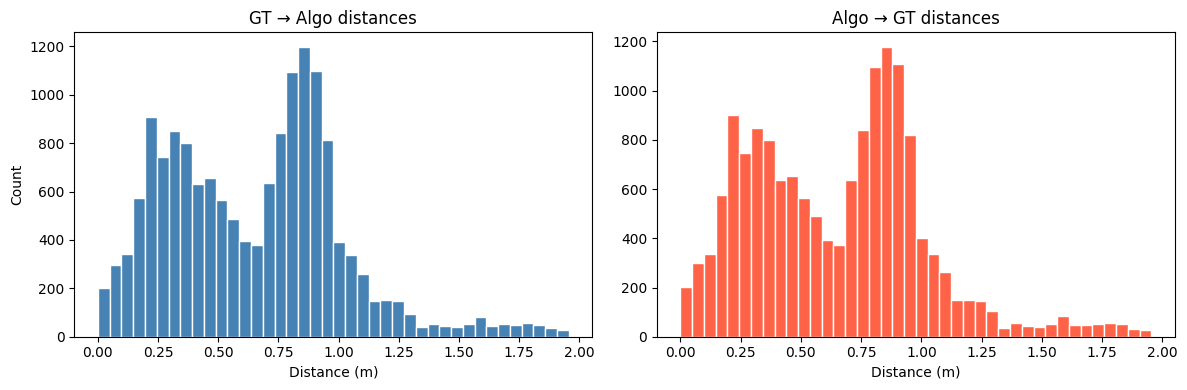
\includegraphics[width=\textwidth]{images/evaluation/trace/hist_wm1}
    \caption{Window Median (Baseline).}
    \label{fig:hist_wm1}
  \end{subfigure}
  \\[0.5em]
  \begin{subfigure}[b]{0.8\textwidth}
    \centering
    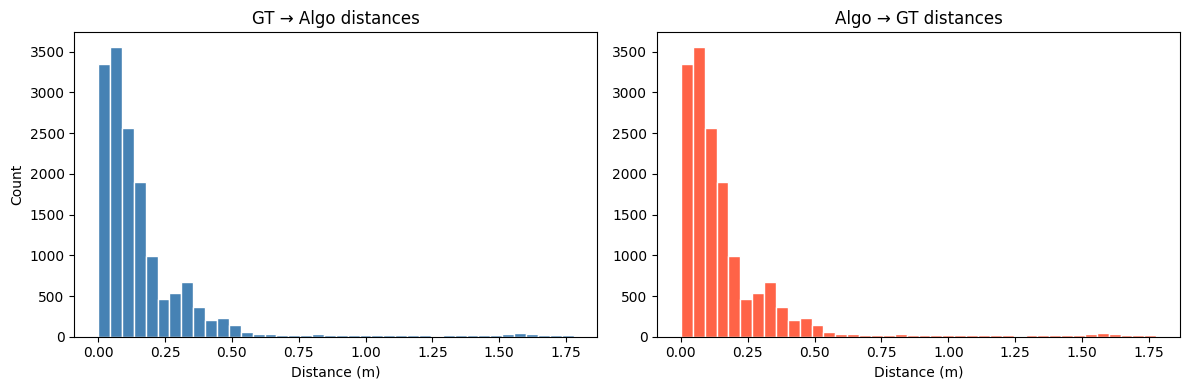
\includegraphics[width=\textwidth]{images/evaluation/trace/hist_wm2}
    \caption{Window Median with Ground Filtering (V2).}
    \label{fig:hist_wm2}
  \end{subfigure}
  \\[0.5em]
  \begin{subfigure}[b]{0.8\textwidth}
    \centering
    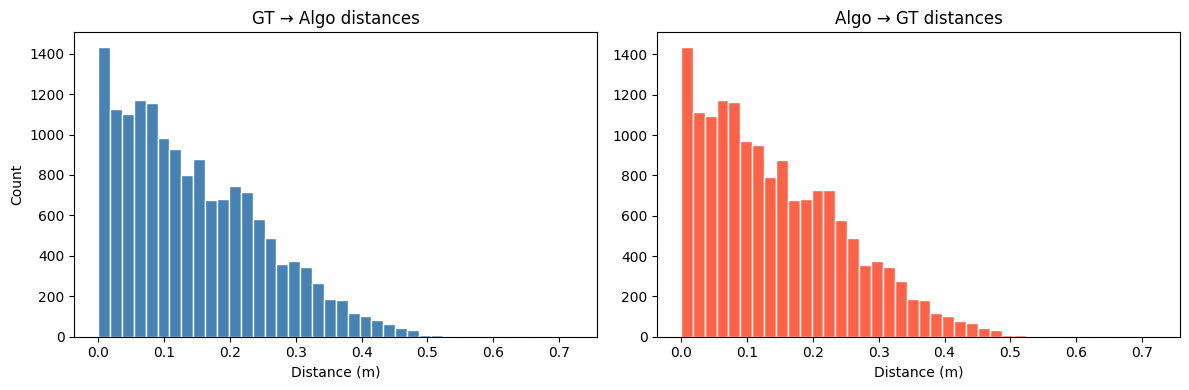
\includegraphics[width=\textwidth]{images/evaluation/trace/hist_pl}
    \caption{Pulse Line Intersection.}
    \label{fig:hist_pl}
  \end{subfigure}
  \\[0.5em]
  \begin{subfigure}[b]{0.8\textwidth}
    \centering
    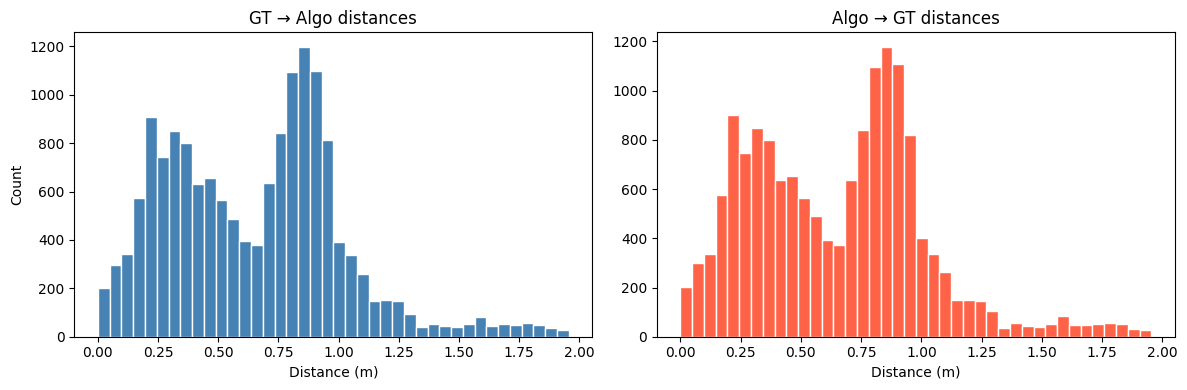
\includegraphics[width=\textwidth]{images/evaluation/trace/hist_cp}
    \caption{Closest Point Convergence.}
    \label{fig:hist_cp}
  \end{subfigure}
  \caption{Distance distribution histograms for all four trajectory reconstruction algorithms. Left: distances from ground-truth sample points to the algorithm trace ($G \to A$); right: distances from algorithm sample points to the ground-truth trace ($A \to G$).}
  \label{fig:trace_histograms}
\end{figure}

\FloatBarrier
\subsection{Summary}
\label{sec:eval_trace_summary}

Among the evaluated methods, the Pulse Line Intersection algorithm achieved the best overall geometric accuracy, with the lowest mean error ($0.147\,\mathrm{m}$), lowest RMSE ($0.182\,\mathrm{m}$), lowest percentile errors, and the smallest Hausdorff distance ($0.725\,\mathrm{m}$). The Window Median V2 algorithm showed a substantial improvement over the baseline Window Median, particularly in average error metrics. The baseline Window Median and Closest Point approaches produced significantly larger deviations, with identical metrics in this evaluation, and higher worst-case errors. These results confirm the selection of Pulse Line Intersection as the default trajectory reconstruction method in the pipeline.

%------------------------------------------------------------------
\section{Lane Extraction Evaluation}
\label{sec:eval_lanes}

\subsection{Evaluated Configurations}
\label{sec:eval_lanes_configs}

To assess the sensitivity of the lane extraction pipeline to key parameters, four configurations were evaluated:

\begin{enumerate}
  \item \textbf{Baseline}: default parameter configuration.
  \item \textbf{Bin\_40}: bin length increased from $25\,\mathrm{units}$ to $40\,\mathrm{units}$.
  \item \textbf{Intensity\_10}: intensity threshold percentile increased from $5\%$ to $10\%$.
  \item \textbf{Intensity\_Kapur}: percentile-based intensity thresholding replaced with max-entropy entropy thresholding.
\end{enumerate}

\paragraph{Note on bin-length units.}\mbox{} \\
The \texttt{bin\_length} parameter is expressed in the native coordinate units of the input point cloud, without any internal reprojection.
In this experiment the input LiDAR data was stored in EPSG:3857 (Web Mercator), whose units are pseudo-metres: at the latitude of the study area (approximately $47^{\circ}$N) the scale factor is $\sec(47^{\circ}) \approx 1.47$, so distances are stretched by roughly $47\%$ relative to true ground distances.
Consequently, the configured values of $25$ and $40$ correspond to approximately $17\,\mathrm{m}$ and $27\,\mathrm{m}$ of actual ground distance, respectively.
Had the input data been provided in a local projected CRS, the same parameter values would directly represent metres on the ground.
All evaluation metrics reported in this chapter are computed after reprojection to EPSG:23700 and therefore reflect true metric distances.

All other pipeline stages and parameters---including input point cloud, temporal window configuration, ground segmentation, road-surface filtering, downsampling, RANSAC line fitting, line smoothing, lane labeling, and output settings---remained identical across all four experiments. This controlled setup ensures that observed performance differences can be attributed directly to the modified parameter.

\subsection{Evaluation Procedure}
\label{sec:eval_lanes_method}

\subsubsection{Cross-Section-Based Matching}

The evaluation compares predicted and ground-truth lane markings using a cross-sectional analysis approach. A set of evenly distributed cross-sections is generated perpendicular to the driving direction along the road segment. For each cross-section, intersections with both the predicted and ground-truth lane lines are computed.

Predicted and ground-truth intersections are then spatially matched based on proximity: a predicted intersection is considered a true positive if it falls within $20\,\mathrm{cm}$ of a ground-truth intersection. This approach evaluates performance at the level of individual lane-marker crossings rather than entire polylines, which directly measures lane count consistency, lateral positional accuracy, and lane-type classification quality. A total of 467 cross-sections were evaluated in each experiment.

\begin{figure}[htbp]
  \centering
  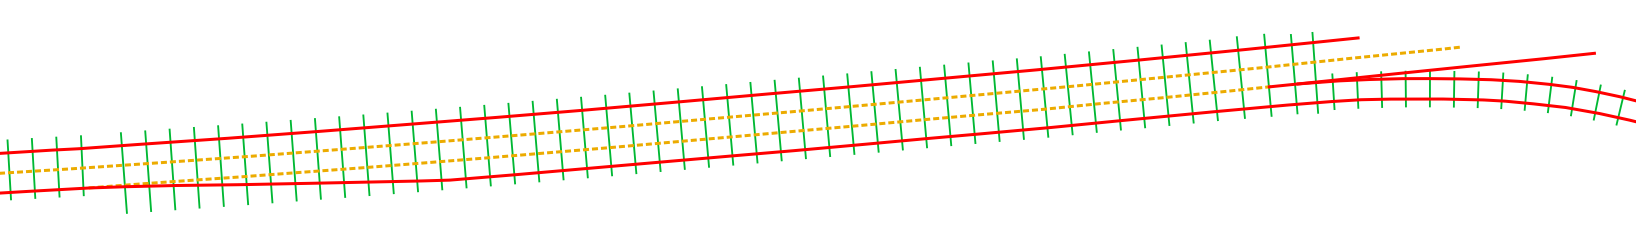
\includegraphics[width=0.7\textwidth]{images/evaluation/lanes/ground_truth_cross_sections}
  \caption{Ground-truth lane geometries: solid lane markings (continuous red), dashed lane markings (dashed orange). The evaluated cross-sections are displayed in green.}
  \label{fig:lbem_cross_section}
\end{figure}

\subsubsection{Detection Metrics}

The following detection metrics were computed from the matched intersections:
\begin{description}
  \item[True Positives (TP)] Predicted intersections correctly matched to a ground-truth intersection.
  \item[False Positives (FP)] Predicted intersections not matched to any ground-truth intersection.
  \item[False Negatives (FN)] Ground-truth intersections not matched by any prediction.
\end{description}

From these counts, standard information-retrieval metrics were derived:
\begin{equation}
  \mathrm{Precision} = \frac{TP}{TP + FP}, \qquad
  \mathrm{Recall} = \frac{TP}{TP + FN}, \qquad
  F_1 = 2 \cdot \frac{\mathrm{Precision} \cdot \mathrm{Recall}}{\mathrm{Precision} + \mathrm{Recall}}.
  \label{eq:prf1}
\end{equation}

\subsubsection{Geometric Accuracy Metrics}

For all matched intersection pairs, the Euclidean distance $d_i$ between the predicted and ground-truth positions was computed. The following statistics were evaluated:
\begin{equation}
  \mu = \frac{1}{N}\sum_{i=1}^{N} d_i, \qquad
  \mathrm{RMSE} = \sqrt{\frac{1}{N}\sum_{i=1}^{N} d_i^2}.
  \label{eq:lane_geo}
\end{equation}
Additionally, the median error, 95th percentile error (P95), and maximum error were reported.

\subsubsection{Lane Classification and Topological Metrics}

Each matched pair was compared by semantic class (solid or dashed). Classification accuracy measures, among the spatially matched intersection pairs, the fraction whose predicted lane type (solid or dashed) agrees with the ground-truth label:
\begin{equation}
  \mathrm{Acc}_{\mathrm{class}} = \frac{|\{i : \hat{y}_i = y_i\}|}{TP},
  \label{eq:class_acc}
\end{equation}
where $\hat{y}_i$ is the predicted semantic class and $y_i$ is the ground-truth class of the $i$-th matched pair. Purely spatial proximity is not sufficient for a correct prediction: the lane type must also match. For topological consistency, the lane count mean absolute error (MAE) was computed:
\begin{equation}
  \mathrm{MAE}_{\mathrm{count}} = \frac{1}{N}\sum_{i=1}^{N} |p_i - g_i|,
  \label{eq:lane_count_mae}
\end{equation}
where $p_i$ and $g_i$ denote the predicted and ground-truth lane counts at cross-section~$i$. The percentage of cross-sections where $p_i = g_i$ exactly (perfect cross-sections) was also reported.

\FloatBarrier
\subsection{Evaluation Results}
\label{sec:eval_lanes_results}

Table~\ref{tab:lane_eval} summarizes the evaluation results for all four configurations.

\begin{table}[htbp]
  \centering
  \caption{Lane extraction evaluation results across the four parameter configurations.}
  \label{tab:lane_eval}
  \small
  \begin{tabular}{@{}lrrrr@{}}
    \hline
    Metric & Baseline & Bin\_40 & Intensity\_10 & Intensity\_Kapur \\
    \hline
    TP                            & 1374   & 1348   & 1360   & 1374   \\
    FP                            & 1      & 13     & 14     & 4      \\
    FN                            & 20     & 46     & 34     & 20     \\
    Precision                     & 0.9993 & 0.9904 & 0.9898 & 0.9971 \\
    Recall                        & 0.9857 & 0.9670 & 0.9756 & 0.9857 \\
    $F_1$                         & 0.9924 & 0.9786 & 0.9827 & 0.9913 \\
    \hline
    Mean error (m)                & 0.0213 & 0.0221 & 0.0228 & 0.0220 \\
    RMSE (m)                      & 0.0280 & 0.0293 & 0.0307 & 0.0292 \\
    Median error (m)              & 0.0166 & 0.0175 & 0.0172 & 0.0173 \\
    P95 error (m)                 & 0.0564 & 0.0593 & 0.0589 & 0.0585 \\
    Max error (m)                 & 0.1750 & 0.1791 & 0.1832 & 0.1754 \\
    \hline
    Classification accuracy       & 0.9993 & 0.9993 & 0.9971 & 0.9993 \\
    Lane count MAE                & 0.0407 & 0.0707 & 0.0428 & 0.0471 \\
    Perfect cross-sections (\%)   & 96.36  & 93.15  & 96.15  & 95.72  \\
    Cross-sections                & 467    & 467    & 467    & 467    \\
    \hline
  \end{tabular}
\end{table}

\FloatBarrier
\subsection{Discussion}
\label{sec:eval_lanes_discussion}

The baseline configuration achieved the best overall performance across nearly all evaluation metrics: highest $F_1$ score ($0.9924$), lowest geometric errors, lowest lane-count MAE ($0.0407$), and the highest percentage of perfectly reconstructed cross-sections ($96.36\%$). These results indicate that the original parameter configuration provides the best balance between detection sensitivity, geometric precision, and topological consistency.

\begin{figure}[htbp]
  \centering
  \begin{subfigure}[b]{0.85\textwidth}
    \centering
    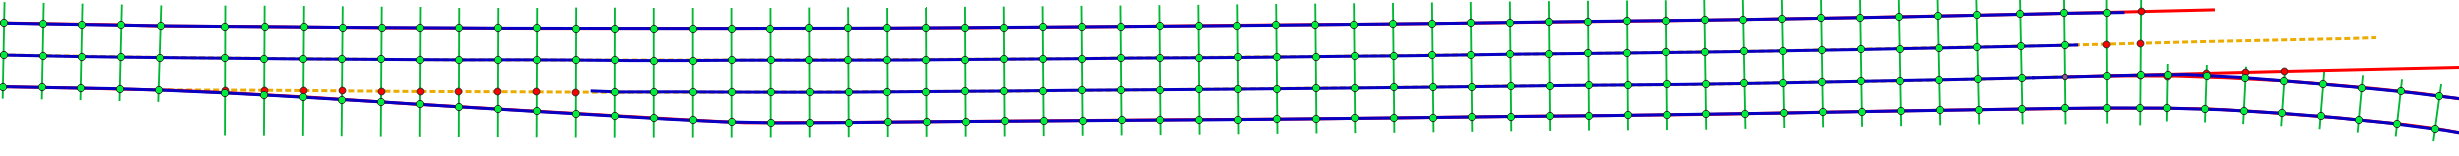
\includegraphics[width=\textwidth]{images/evaluation/lanes/eval_points}
    \caption{A road section where lane lines merge and split: the line-fitting stage cannot correctly handle such topological changes, resulting in false negatives.}
    \label{fig:eval_points_merge}
  \end{subfigure}
  \\[0.5em]
  \begin{subfigure}[b]{0.85\textwidth}
    \centering
    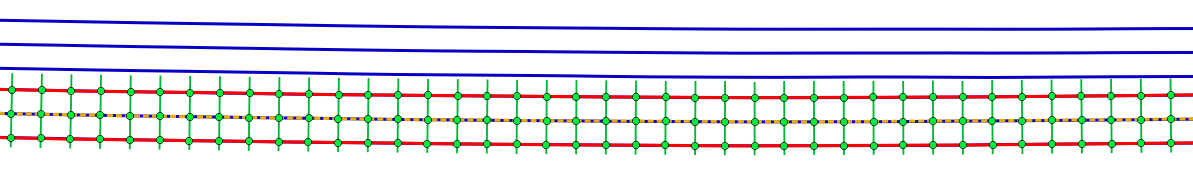
\includegraphics[width=\textwidth]{images/evaluation/lanes/eval_points_2}
    \caption{A typical highway section with no merging or splitting: all four configurations performed well under these ordinary conditions.}
    \label{fig:eval_points_normal}
  \end{subfigure}
  \caption{Qualitative evaluation results. Ground-truth solid markings (solid red), ground-truth dashed markings (dashed orange), extracted lane geometries (blue); true positives with correct semantic match (green dots), false negatives (red dots).}
  \label{fig:eval_points}
\end{figure}

The Kapur thresholding configuration (\textit{Intensity\_Kapur}) produced performance very close to the baseline. Although it introduced slightly more false positives (4 vs.\ 1), recall remained identical, and the geometric accuracy degradation was minimal. This suggests that entropy-based thresholding is a viable alternative to percentile-based intensity filtering and may be preferable in scenarios where the intensity distribution is less predictable.

Increasing the intensity percentile threshold to $10\%$ (\textit{Intensity\_10}) reduced detection quality: more false positives and false negatives were produced, leading to lower precision ($0.9898$), recall ($0.9756$), and $F_1$ score ($0.9827$). Geometric error metrics also increased slightly, indicating that the higher threshold likely suppresses valid lane marking points while retaining noise, making accurate line fitting more difficult.

The weakest performance was observed in the increased bin-length configuration (\textit{Bin\_40}). Enlarging the temporal bin length from $25$ to $40$ Web Mercator pseudo-metres (approximately $17\,\mathrm{m}$ to $27\,\mathrm{m}$ on the ground) substantially reduced recall ($0.9670$) and introduced the most false positives and lane-count inconsistencies. The decrease in perfect cross-sections ($93.15\%$) and the increased lane-count MAE ($0.0707$) indicate degraded topological reconstruction quality. This suggests that larger binning regions reduce the pipeline's ability to adapt to local road geometry variations and lane-structure changes.

Overall, the experiments demonstrate that the pipeline is highly sensitive to the binning configuration and moderately sensitive to intensity-threshold selection. Across all tested configurations, the baseline achieves sub-centimetre mean positional accuracy ($2.1\,\mathrm{cm}$) and near-perfect lane detection ($F_1 > 0.99$), confirming the effectiveness of the proposed lane extraction approach.

\FloatBarrier
\section{Performance and Resource Usage}
\label{sec:eval_performance}

All experiments were executed on an Apple MacBook Pro (Mac15,7) with an Apple M3 Pro SoC containing 12 CPU cores (6 performance and 6 efficiency cores) and $36,\mathrm{GB}$ of unified memory.

\subsection{Stage-wise Runtime}
Table~\ref{tab:stage_times} reports the average runtime (over 10 runs) for each pipeline stage when processing a typical highway segment.

\begin{table}[htbp]
  \centering
  \caption{Average runtime per pipeline stage (10 runs).}
  \label{tab:stage_times}
  \small
  \begin{tabular}{@{}lr@{}}
    \hline
    \textbf{Stage} & \textbf{Time (s)} \\
    \hline
    Setup Stage & 2.45 \\
    Car Trace Stage & 4.56 \\
    Binning Stage (1st) & 15.29 \\
    TraceDistanceFilterStage & 0.90 \\
    GroundSegmentStage & 14.18 \\
    IntensityThresholdStage & 11.22 \\
    RoadSurfaceFilter & 4.85 \\
    DownsampleStage & 3.32 \\
    Binning Stage (2nd) & 0.07 \\
    FitLinesStage & 10.47 \\
    LineSmoothingStage & 16.41 \\
    LineLabelingStage & 31.19 \\
    \hline
  \end{tabular}
\end{table}

The total runtime for a full pipeline execution is approximately 115 seconds (just under 2 minutes) for a ~5 km highway segment, and more than 100 million points.

\subsection{Point Cloud Size Reduction}
The pipeline achieves substantial data reduction through progressive filtering and downsampling. Table~\ref{tab:point_reduction} shows the number of points remaining after each major stage for the sample tile 871e1d886ffffff.

\begin{table}[htbp]
  \centering
  \caption{Point count after each major processing stage (tile 871e1d886ffffff).}
  \label{tab:point_reduction}
  \small
  \begin{tabular}{@{}lr@{}}
    \hline
    \textbf{Stage} & \textbf{Points Remaining} \\
    \hline
    Raw input & 104,028,999 \\
    Distance clip & 81,139,327 \\
    Ground segmentation & 60,822,026 \\
    Intensity thresholding & 3,317,369 \\
    Road surface extraction & 894,671 \\
    Downsampling & 342,185 \\
    \hline
  \end{tabular}
\end{table}

This reduction enables efficient downstream processing and storage, while preserving all relevant lane geometry information.
